\documentclass{article}
\usepackage{polski}
\usepackage[utf8]{inputenc}
\usepackage{float}
\usepackage{graphicx}
\usepackage{caption}
\usepackage{subcaption}
\usepackage{ragged2e}
\usepackage{amsmath}
\usepackage{amssymb}
\usepackage{amsfonts}
\usepackage{blindtext}
\usepackage{hyperref}
\usepackage{algorithmicx}
\usepackage{listings}
\usepackage{booktabs}
\usepackage{siunitx}
\usepackage{multicol}
\usepackage{fancyvrb}
\usepackage{algpseudocode}
\usepackage{algorithm}

\begin{document}

\AddToHook{cmd/section/before}{\clearpage}

\section*{Zadanie 1}
\subsubsection*{Opis metody}
Metoda bisekcji znajduje miejsce zerowe dla funkcji ciągłej
$f(x)$, która zmienia znak na końcach danego przedziału $[a,b]$.
Polega ona na ciągłym dzieleniu przedziału na dwa mniejsze przedziały
i wybraniu tego, w którym funkcja nadal zmienia znak.
W ten sposób otrzymujemy coraz to mniejsze
przedziały, w których znajduje się miejsce zerowe.
Powtarzamy ten proces aż do spełnienia warunków końcowych.

\subsubsection*{Warunki końcowe}
Metodę kończymy gdy długość przedziału jest mniejsza od zadanego
$\delta$ lub gdy wartość po środku jest co do modułu
mniejsza od zadanego $\epsilon$.

\subsubsection*{Zbieżność i złożoność metody}
Metoda bisekcji jest zbieżna globalnie. Jedynym warunkiem jej działania
dla przedziału, który zawiera miejsce zerowe i w którym funkcja zmienia
znak jest to, aby funkcja była ciągła.

Ponadto jeżeli ograniczymy się do $\delta$ to znalezienie miejsca
zerowego wymaga dokładnie
\[
  \lceil\log_2(\frac{b-a}{\delta})\rceil - 1
\] iteracji.

\subsubsection*{Zwracane wartości}
Jeśli funkcja nie zmienia znaku na końcach przedziału, to
nie możemy zastosować tej metody. Wtedy zwracamy kod błędu 1.
W przeciwnym wypadku zwracamy wynik wraz z kodem błędu 0.

\clearpage
\subsubsection*{Pseudokod}
\begin{algorithm}[H]
  \caption{Bisection Method for Finding Function Roots}
  \begin{algorithmic}[1]
  \Procedure{MBisekcji}{$f, a, b, \delta, \epsilon$}
      \If{$\text{sign}(f(a)) = \text{sign}(f(b))$}
          \State \Return Nil, Nil, Nil, 1
      \EndIf
      \State $it \gets 1$
      \While{True}
          \State $c \gets (a + b) / 2$
          \State $f_c \gets f(c)$
          \If{$f_c = 0$ \textbf{or} $(b - a) / 2 < \delta$ \textbf{or} $\left| f_c \right| < \epsilon$}
              \State \Return $c, f_c, it, 0$
          \EndIf
          \State $it \gets it + 1$
          \If{$\text{sign}(f_c) = \text{sign}(f(a))$}
              \State $a \gets c$
          \Else
              \State $b \gets c$
          \EndIf
      \EndWhile
  \EndProcedure
  \end{algorithmic}
  \end{algorithm}


\subsubsection*{Wizualizacja}
\begin{figure}[H]
  \centering
  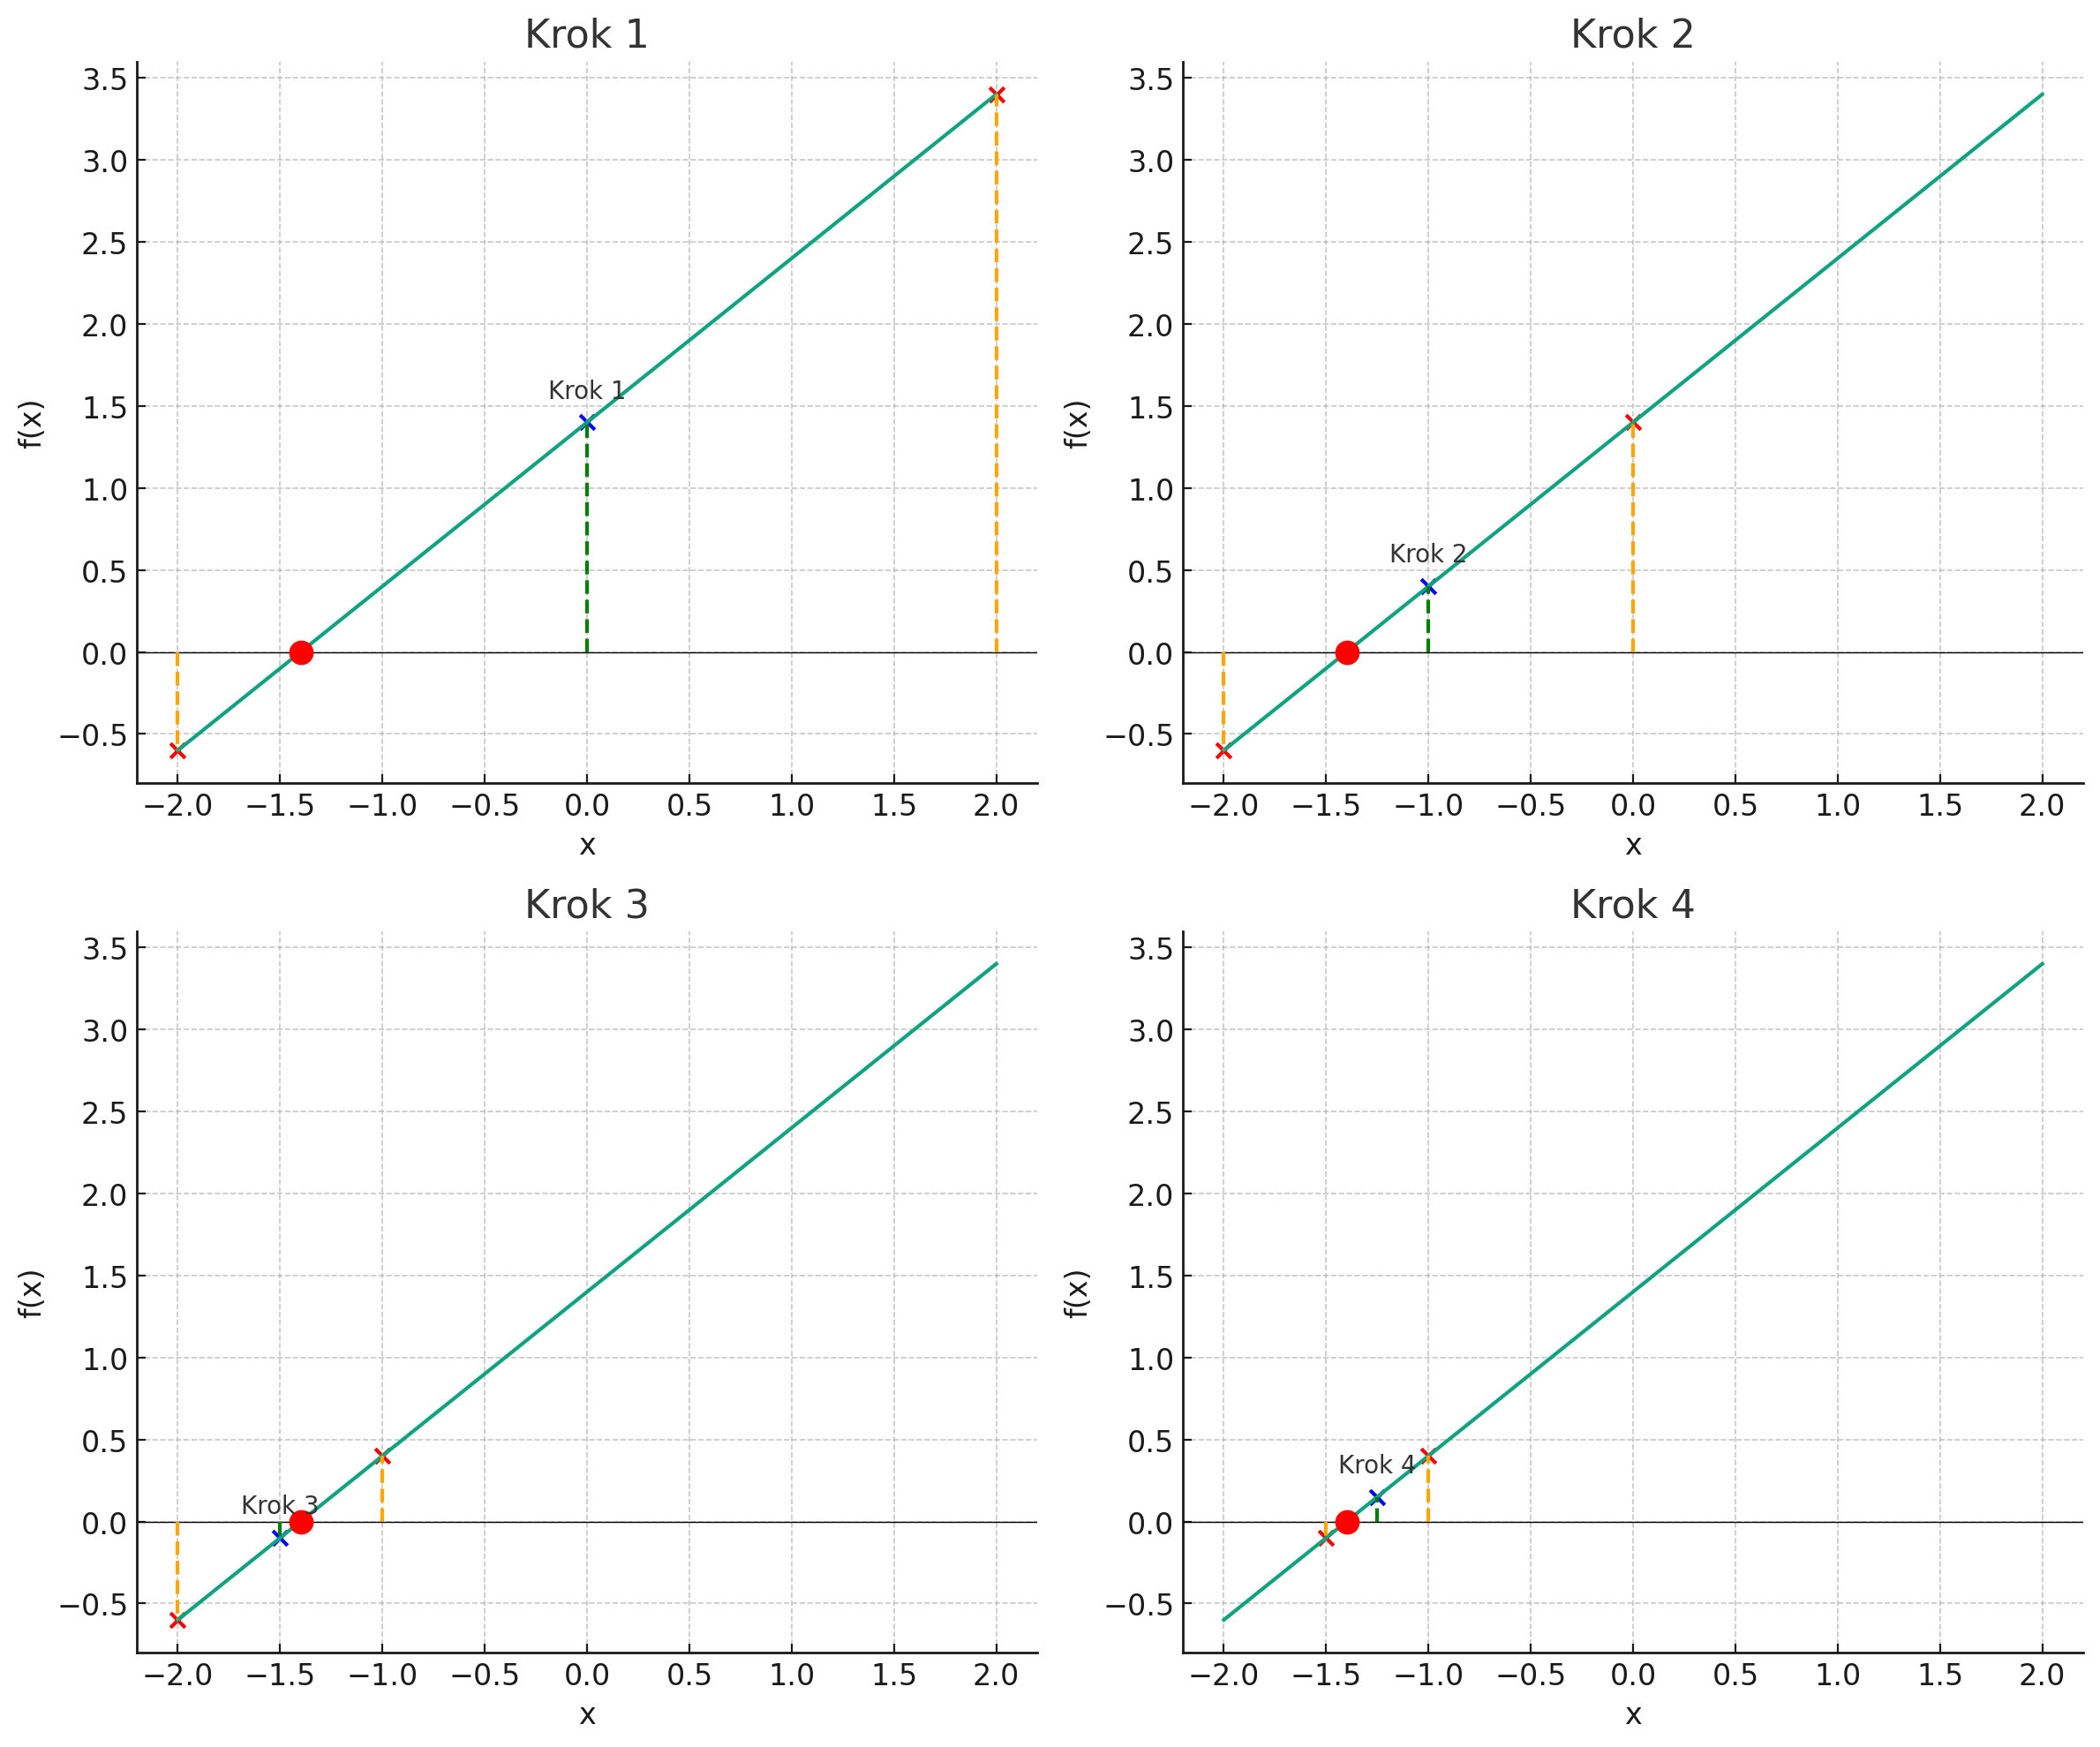
\includegraphics[width=\textwidth]{./ex1.png}
  \caption{Wizualizacja pierwszych czterech kroków dla $f(x) = x + 1.4$.}
\end{figure}




\section*{Zadanie 2}
\subsubsection*{Opis metody}
Metoda stycznych, zwana także metodą Newtona jest metodą
numeryczną szukającą miejsca zerowego dla danej funkcji $f(x)$.
Poza samą funkcją
$f(x)$ wymaga również znajomości jej pochodnej $f'(x)$. Metoda
polega na wyznaczeniu stycznej do wykresu funkcji $f(x)$ w punkcie
$x_0$. Następnie znajdujemy punkt przecięcia się tej stycznej z osią
$x$. W ten sposób otrzymujemy nowy punkt $x_1$.
W ten sposób otrzymujemy coraz
to lepsze przybliżenia miejsca zerowego funkcji $f(x)$.
Powtarzamy ten proces aż do spełnienia warunków końcowych.

\subsubsection*{Warunki końcowe}
Metodę kończymy gdy wartość bezwzględna różnicy między kolejnymi
przybliżeniami jest mniejsza od zadanego $\delta$.

\subsubsection*{Zbieżność i złożoność metody}
Metoda jest zbieżna lokalnie, a nie globalnie, przez to musimy
zadbać o to, aby punkt startowy $x_0$ był odpowiednio dobrany.
W przeciwnym wypadku metoda może nie zbiegać do rozwiązania.
Z tego powodu nakładamy również ograniczenie na maksymalną liczbę iteracji.
Metoda jest zbieżna kwadratowo, co oznacza, że z każdą iteracją
liczba cyfr dokładnych przybliżenia podwoi się. Nigdy też nie wykonamy
więcej iteracji niż nałożone ograniczenie $it_{max}$.

\subsubsection*{Zwracane wartości}
Jeśli nie udało się znaleźć miejsca zerowego w maksymalnej liczbie iteracji, to
zwracamy kod błędu 1. Kolejnym zagrożeniem jest to, że pochodna może
być zbyt bliska 0. W praktyce oznacza to, że co do modułu jest ona
mniejsza niż dane $\epsilon$. Wtedy metoda zwraca kod błędu 2.
Jeśli nie zaszła żadna z powyższych sytuacji, zwracamy wynik
wraz z kodem błędu 0.

\subsubsection*{Pseudokod}
\begin{algorithm}[H]
  \caption{Method of Tangents (Newton's Method) for Finding Function Roots}
  \begin{algorithmic}[1]
  \Procedure{MStycznych}{$f, pf, x_0, \delta, \epsilon, \text{maxit}$}
      \State $it \gets 1$
      \State $x \gets x_0$
      \While{$it < \text{maxit}$}
          \State $y \gets f(x)$
          \State $y' \gets pf(x)$
          \If{$\left| y' \right| < \epsilon$}
              \State \Return $x, y, it, 2$
          \EndIf
          \State $x_1 \gets x - \frac{y}{y'}$
          \If{$\left| x_1 - x \right| < \delta$}
              \State \Return $x_1, f(x_1), it, 0$
          \EndIf
          \State $x \gets x_1$
          \State $it \gets it + 1$
      \EndWhile
      \State \Return $x, f(x), it, 1$
  \EndProcedure
  \end{algorithmic}
  \end{algorithm}

\subsubsection*{Wizualizacja}
\begin{figure}[H]
  \centering
  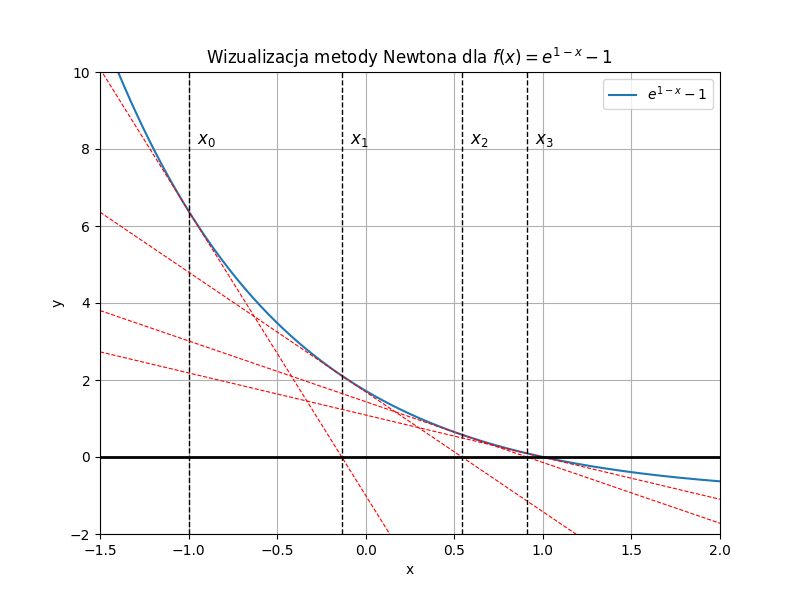
\includegraphics[width=\textwidth]{./ex2.png}
  \caption{Wizualizacja pierwszych trzech kroków dla $f(x) = e^{1-x} - 1$.}
\end{figure}



\section*{Zadanie 3}
\subsubsection*{Opis metody}
Metoda siecznych jest podobna do metody stycznych, ale zamiast
stycznej wyznaczamy prostą przechodzącą przez dwa punkty. Dzięki
temu nie musimy wpierw wyznaczać pochodnej funkcji $f(x)$. Ze względu
na charakterystykę funkcji potrzebujemy dwóch punktów startowych
$x_0$ oraz $x_1$.

\subsubsection*{Warunki końcowe}
Jako warunki końcowe przyjąłem
\[
|x_2 - x_1| < \delta \text{{ lub }} |f(x_1)| < \epsilon
\]
gdzie $x_2$ jest kolejnym przybliżeniem miejsca zerowego.
\[
x_2 = x_1 - \frac{f(x_1)(x_1 - x_0)}{f(x_1) - f(x_0)}
\]

\subsubsection*{Zbieżność i złożoność metody}
Podobnie jak metoda Newtona metoda siecznych jest zbieżna lokalnie.
Jej wykładnik zbieżności wynosi $\frac{1 + \sqrt{5}}{2} \approx 1.618$.
Czyli jest ona wolniejsza od metody Newtona, ale szybsza od metody bisekcji.

\subsubsection*{Zwracane wartości}
Jeśli udało nam się znaleźć miejsce zerowe, to zwracamy je wraz z
wartością funkcji w tym punkcie, liczbą iteracji oraz kodem błędu 0.
Jeśli natomiast nie udało się znaleźć miejsca zerowego w maksymalnej
liczbie iteracji, to zwracamy kod błędu 1.

\subsubsection*{Pseudokod}
\begin{algorithm}[H]
  \caption{Secant Method for Finding Function Roots}
  \begin{algorithmic}[1]
  \Procedure{MSiecznych}{$f, x_0, x_1, \delta, \epsilon, \text{maxit}$}
      \State $it \gets 1$
      \While{$it < \text{maxit}$}
          \State $x_2 \gets x_1 - f(x_1) \times \frac{x_1 - x_0}{f(x_1) - f(x_0)}$
          \If{$\left| x_2 - x_1 \right| < \delta$ \textbf{or} $\left| f(x_1) \right| < \epsilon$}
              \State \Return $x_2, f(x_2), it, 0$
          \EndIf
          \State $x_0 \gets x_1$
          \State $x_1 \gets x_2$
          \State $it \gets it + 1$
      \EndWhile
      \State \Return $x_1, f(x_1), it, 1$
  \EndProcedure
  \end{algorithmic}
  \end{algorithm}

\subsubsection*{Wizualizacja}
\begin{figure}[H]
  \centering
  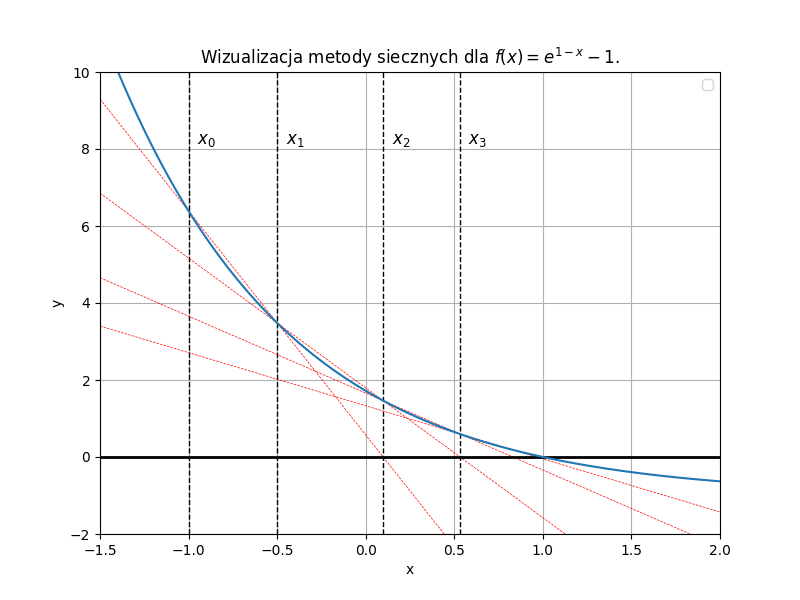
\includegraphics[width=\textwidth]{./ex2_2.png}
  \caption{Wizualizacja pierwszych trzech kroków dla $f(x) = e^{1-x} - 1$.}
\end{figure}



\section*{Zadanie 4}
W tym zadaniu dane mamy
\begin{gather*}
f(x) = \sin(x) - {(\frac{1}{2}x)}^2\\
\delta = \frac{1}{2}10^{-5}\\
\epsilon = \frac{1}{2}10^{-5}
\end{gather*}
chcemy wyznaczyć miejsca zerowe $f$ następującymi metodami:
\begin{enumerate}
  \item metoda biskecji na przedziale $[1.5, 2.0]$
  \item metoda stycznych dla $x_0=1.5$
  \item metoda siecznych dla $x_0=1$, $x_1=2$
\end{enumerate}
\subsection*{wyniki}
\begin{table}[h]
  \centering
  \begin{tabular}{|l|l|l|l|l|}
  \hline
  \textbf{Metoda}      & \textbf{x}              & \textbf{f(x)}                   & \textbf{it} & \textbf{err} \\ \hline
  Bisekcji             & 1.9337539672851562      & -2.7027680138402843e-7          & 16          & 0            \\ \hline
  Stycznych            & 1.9337537628270214      & -2.220446049250313e-16          & 5           & 0            \\ \hline
  Siecznych            & 1.933753759901896       & 3.8667741231179775e-9           & 4           & 0            \\ \hline
  \end{tabular}
  \caption{Porównanie wyników dla $f(x)=\sin(x)-{(\frac{1}{2}x)}^2$}
\end{table}
Widzimy, że wszystkie metody zwróciły poprawne wyniki.
Metoda bisekcji była zdecydowanie najwolniejsza, potrzebowała
aż 16 iteracji, aby osiągnąć wynik. Najszybsza okazała się metoda
siecznych, która potrzebowała tylko 4 iteracji pomimo teoretycznie
mniejszego wykładnika zbieżności od metody Newtona.


\section*{Zadanie 5}
Dane mamy
\begin{gather*}
f(x)=3x\\
g(x)=e^x\\
\delta=10^{-4}\\
\epsilon=10^{-4}
\end{gather*}
Chcemy wyznaczyć miejsce przecięcia funkcji $f(x)$ oraz $g(x)$
metodą biskecji, co jest równoważne z rozwiązaniem równania $f(x)-g(x)=0$.
\begin{figure}[H]
  \centering
  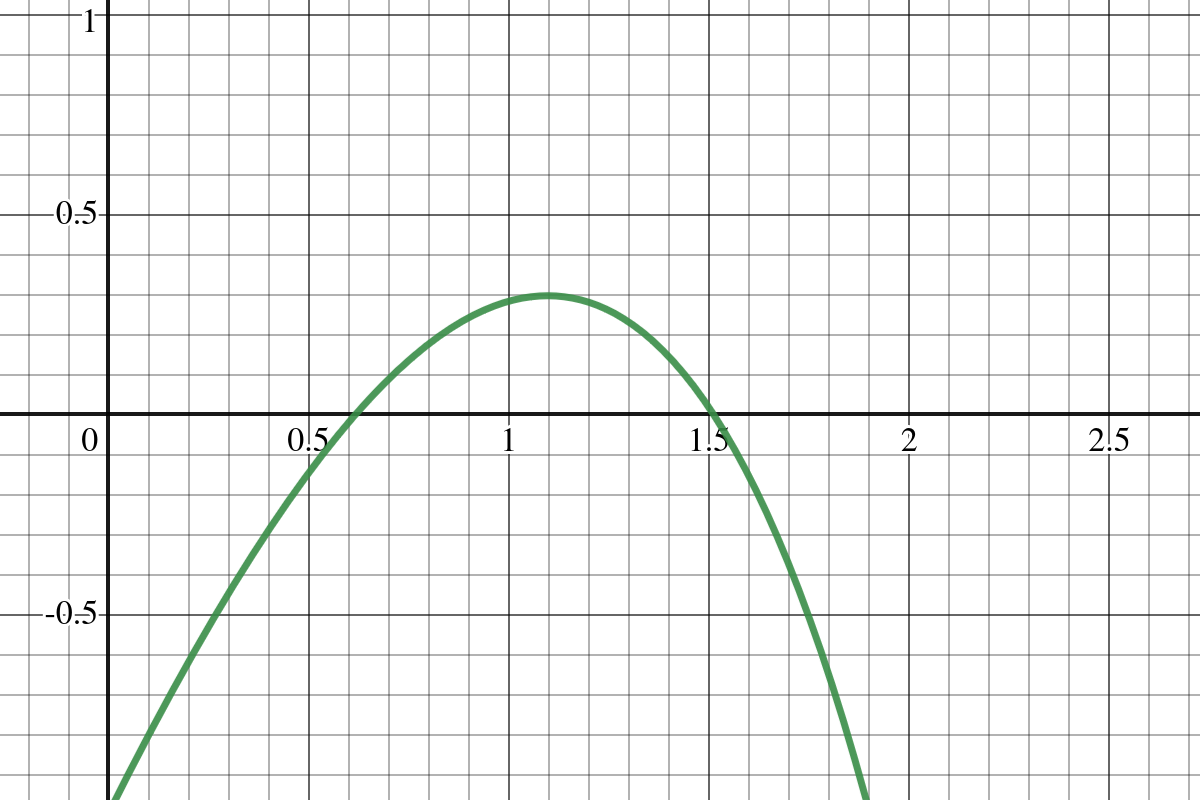
\includegraphics[width=\textwidth]{./ex5.png}
  \caption{Wykres $f(x)-g(x)$}
\end{figure}
Na wykresie widzimy, że funkcja ma dwa miejsca zerowe.
Musimy więc zastosować metodę bisekcji dwukrotnie.
\begin{table}[h]
  \centering
  \begin{tabular}{|l|l|l|l|l|}
  \hline
  \textbf{x}            & \textbf{f(x)}                      & \textbf{it} & \textbf{err} \\ \hline
  0.619140625           & -9.066320343276146e-5              & 9           & 0            \\ \hline
  1.5120849609375       & -7.618578602741621e-5              & 13          & 0            \\ \hline
  \end{tabular}
  \caption{Znalezione przybliżenia miejsc zerowych dla $f(x)-g(x)$}
\end{table}
Udało nam się znaleźć przybliżenia obu miejsc zerowych. Warto jednak
zwrócić uwagę na to, że bez uprzedniej wiedzy o tym ile tych miejsc jest
oraz w jakich przedziałach się znajdują, nie bylibyśmy w stanie
zastosować metody bisekcji.



\section*{Zadanie 6}
Mamy dane
\begin{gather*}
f_1(x) = e^{1-x} - 1\\
f_2(x) = xe^{-x}\\
\delta = 10^{-5}\\
\epsilon = 10^{-5}
\end{gather*}
Chcemy wyznaczyć miejsca zerowe funkcji $f_1$ oraz $f_2$.

\subsection*{funkcja \boldmath{$f_1$}}
\begin{figure}[H]
  \centering
  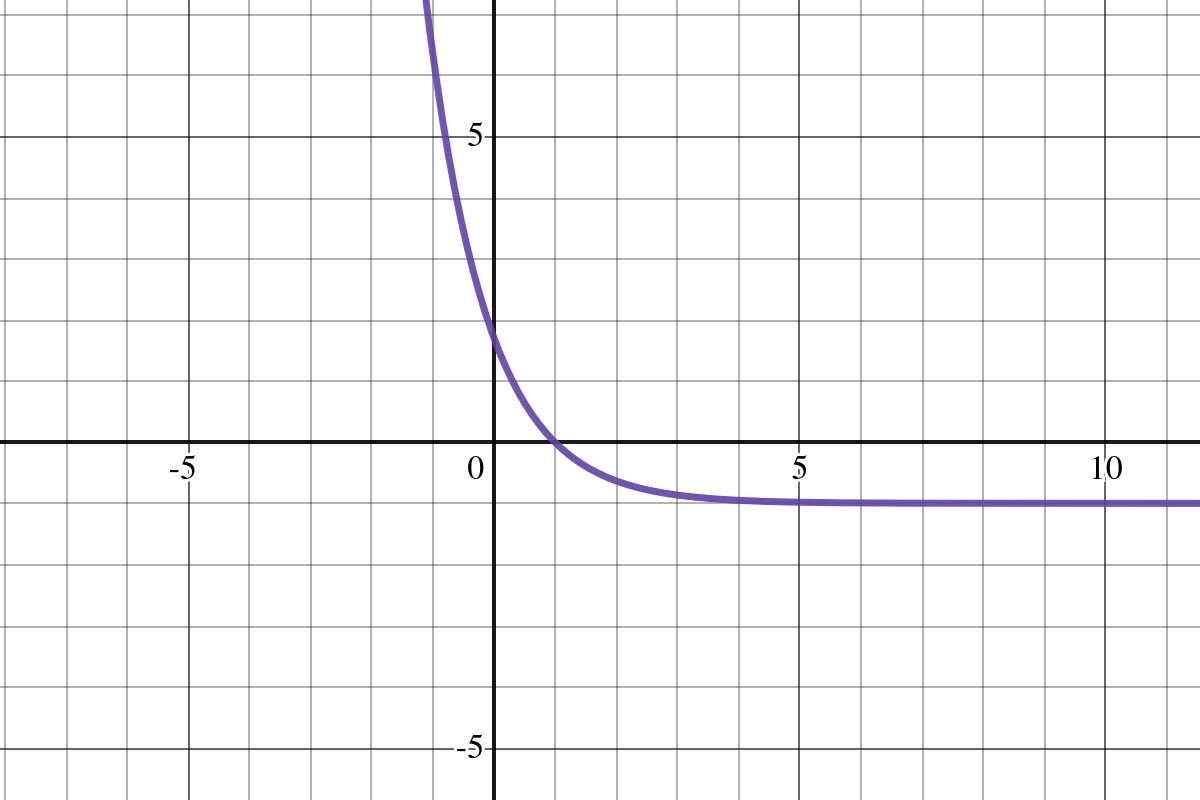
\includegraphics[width=\textwidth]{./ex6f1.png}
  \caption{Funkcja $f_1$}
\end{figure}
Łatwo zauważyć, że funkcja $f_1$ ma jedno miejsce zerowe
$f_1(1) = 0$. Ponadto w nieskończoności funkcja dąży do $-1$,
a w minus nieskończoności do nieskończoności.
\begin{gather*}
  \lim_{x \to \infty} f_1(x) = \lim_{x \to \infty} e^{1-x} - 1 = 0 - 1 = -1\\
  \lim_{x \to -\infty} f_1(x) = \lim_{x \to -\infty} e^{1-x} - 1 = \infty - 1 = \infty
\end{gather*}

\subsubsection*{metoda bisekcji}
Ponieważ miejsca zerowe mają wartość całkowitą, możemy
zastosować metodę bisekcji na przedziałach symetrycznych
względem miejsca zerowego. Wtedy już w pierwszej iteracji
znajdziemy dokładne rozwiązanie. Rozważmy jednak także kilka
innych przedziałów.
\begin{table}[H]
\centering
\begin{tabular}{|l|l|l|l|l|l|}
\hline
\textbf{Przedział}                     & \textbf{x}                    & \textbf{f(x)}                    & \textbf{it} & \textbf{err} \\ \hline
[0.0, 2.0]                            & 1.0                           & 0.0                              & 1           & 0            \\ \hline
[0.0, 1.0]                            & 0.9999923706054688            & 7.629423635080457e-6             & 17          & 0            \\ \hline
[-2.0, 1.0]                           & 0.9999942779541016            & 5.722062269342132e-6             & 19          & 0            \\ \hline
[0.0, 1.0e10]                         & 1.000000082740371             & -8.2740367557399e-8              & 49          & 0            \\ \hline
[$-11^{10}$, 1.0]               & 0.9999942407348015            & 5.759281783035419e-6             & 52          & 0            \\ \hline
[2.0, 3.0]                            & Nothing                       & Nothing                          & Nothing     & 1            \\ \hline
\end{tabular}
\caption{Metoda bisekcji dla \( f_1(x) \)}
\end{table}
Widzimy, że nawet dla bardzo dużych przedziałów metoda bisekcji
znajduje rozwiązanie w mniej niż 50 iteracji. Wynika to z tego,
że złożoność funkcji rośnie jedynie logarytmicznie. Widzimy także, że
rozwiązania nie jesteśmy w stanie znaleźć tylko jeśli nie znajduje
się ono w rozpatrywanym przedziale lub też funkcja nie zmienia
znaku w miejscu zerowym.
  
\subsubsection*{metoda Newtona}
\begin{table}[H]
  \centering
  \begin{tabular}{|l|l|l|l|l|l|}
  \hline
  \boldmath{$x_0$}            & \textbf{x}                   & \textbf{f(x)}                 & \textbf{it} & \textbf{err} \\ \hline
  1.0                    & 1.0                          & 0.0                           & 1           & 0            \\ \hline
  0.0                    & 0.9999999999987766           & 1.2234657731369225e-12        & 5           & 0            \\ \hline
  -5.0                   & 1.0                          & 0.0                           & 11          & 0            \\ \hline
  2.0                    & 0.9999999999999999           & 2.220446049250313e-16         & 6           & 0            \\ \hline
  3.0                    & 0.9999999999999996           & 4.440892098500626e-16         & 10          & 0            \\ \hline
  4.0                    & 1.0                          & 0.0                           & 22          & 0            \\ \hline
  5.0                    & 0.9999999999999362           & 6.394884621840902e-14         & 55          & 0            \\ \hline
  6.0                    & 0.9999999999999991           & 8.881784197001252e-16         & 148         & 0            \\ \hline
  7.0                    & 0.9999999999999986           & 1.5543122344752192e-15        & 402         & 0            \\ \hline
  7.215                  & 1.0                          & 0.0                           & 499         & 0            \\ \hline
  8.0                    & NaN                          & NaN                           & 500         & 1            \\ \hline
  100.0                  & 100.0                        & -1.0                          & 1           & 2            \\ \hline
  -800.0                 & NaN                          & NaN                           & 500         & 1            \\ \hline
  \end{tabular}
  \caption{Metoda Newtona dla \( f_1(x) \)}
\end{table}
Widzimy, że metoda Newtona jest bardzo wrażliwa na wybór punktu
startowego. Gdy wybieramy punkt $x_0$, który jest ujemny i duży
co do modułu, to wartość pochodnej staje się zbyt duża do reprezentacji
przy pomocy typu Float64. Wtedy funkcja zwraca NaN.

Dla wartości mniejszych od 1, które nie są zbyt duże metoda dość szybko
zbiega do rozwiązania. Dla $x_0 = 1$ dostajemy je w pierwszej iteracji.

Gdy jednak wybieramy $x_0 > 1$ metoda zaczyna zbiegać do rozwiązania
wolniej. Dla $x_0 = 7.215$ potrzebujemy aż 499 iteracji, aby osiągnąć
rozwiązanie. Dla $x_0 = 8$ metoda nie zbiega już do rozwiązania w 500 iteracjach.
Dla wartości jeszcze większych wartość pochodnej jest zbyt mała żebyśmy mogli
przedstawić ją za pomocą typu Float64. Wtedy metoda zwraca kod błędu 2.

\subsubsection*{metoda siecznych}
\begin{table}[h]
  \centering
  \begin{tabular}{|l|l|l|l|l|l|l|}
  \hline
  \textbf{x0}    & \textbf{x1}        & \textbf{x}                   & \textbf{f(x)}                 & \textbf{it} & \textbf{err} \\ \hline
  0.0            & 0.0                & NaN                          & NaN                           & 500         & 1            \\ \hline
  0.0            & 0.5                & 0.999999999991586            & 8.414158259029136e-12         & 6           & 0            \\ \hline
  -0.5           & 0.0                & 0.9999999999886773           & 1.1322720538942121e-11        & 7           & 0            \\ \hline
  3.5            & 6.0                & 0.9999999999927485           & -2.0004225633713348e-9        & 23          & 0            \\ \hline
  500.0          & 500.5              & NaN                          & NaN                           & 500         & 1            \\ \hline
  \end{tabular}
  \caption{Metoda siecznych dla \( f_1(x) \)}
\end{table}
Oczywistym jest, że wybranie punktu $x_0 = x_1$ nie pozwoli nam
znaleźć rozwiązania. Dla wartości bliskich siebie metoda zbiega
do rozwiązania bardzo szybko. Dla $x_0 = 0.0$ oraz $x_1 = 0.5$
potrzebujemy tylko 6 iteracji. Ponieważ funkcja $f_1$ tak szybko
się wypłaszcza dla $x > 1$, to już dla $x_0 = 3.5$ oraz $x_1 = 6.0$
potrzebujemy 23 iteracji, a dla większych wartości funkcja
nie zbiega w limicie 500 iteracji.

\subsection*{funkcja \boldmath{$f_2$}}
\begin{figure}[H]
  \centering
  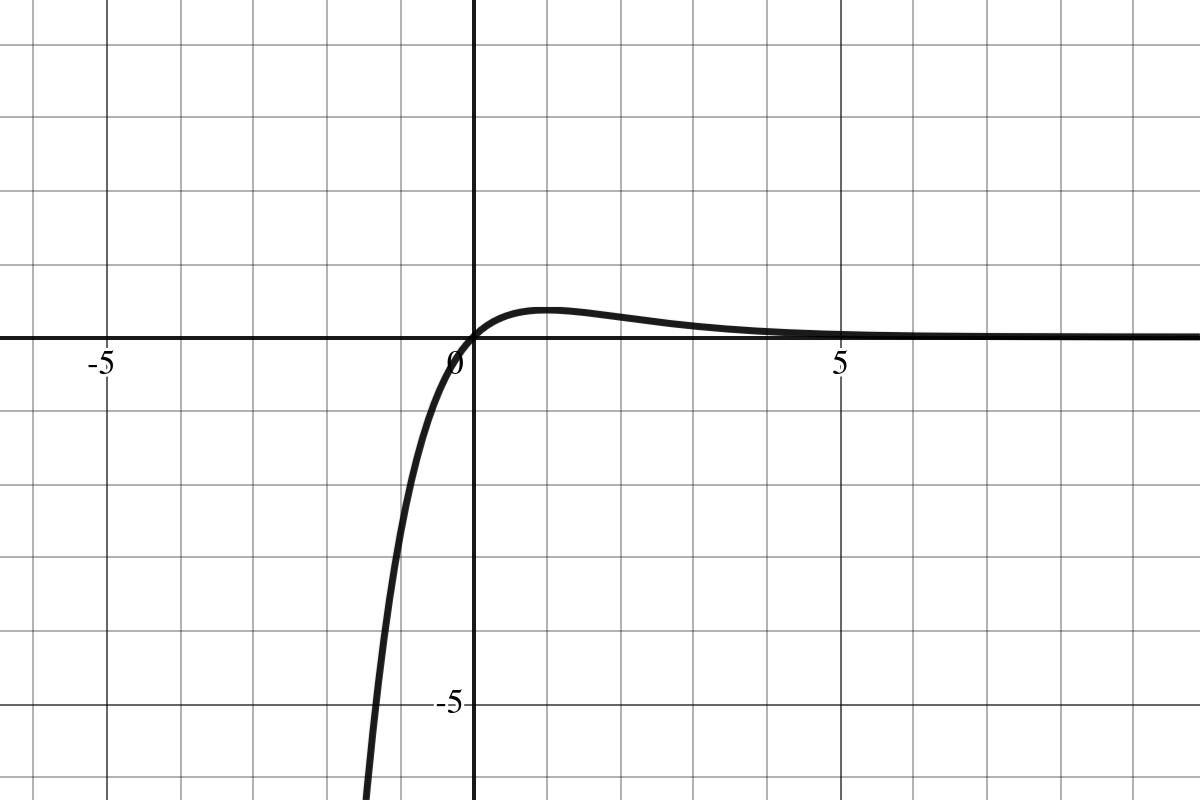
\includegraphics[width=\textwidth]{./ex6f2.png}
  \caption{Funkcja $f_2$}
\end{figure}
Funkcja $f_2$ ma jedno miejsce zerowe $f_2(0) = 0$. Ponadto w nieskończoności
funkcja dąży do $0$, a w minus nieskończoności do $-\infty$.
\begin{gather*}
  \lim_{x \to \infty} f_2(x) = \lim_{x \to \infty} xe^{-x} = \lim_{x \to \infty} \frac{x}{e^x} = 0\\
  \lim_{x \to -\infty} f_2(x) = \lim_{x \to -\infty} xe^{-x} = \lim_{x \to -\infty} \frac{x}{e^x} = -\infty
\end{gather*}

\subsubsection*{metoda bisekcji}
\begin{table}[h]
  \centering
  \begin{tabular}{|l|l|l|l|l|}
  \hline
  \textbf{Przedział}                           & \textbf{x}                    & \textbf{f(x)}                   & \textbf{it} & \textbf{err} \\ \hline
  [-1.0, 1.0]                                 & 0.0                           & 0.0                             & 1           & 0            \\ \hline
  [-5.0, 1.0]                                 & -7.62939453125e-6             & -7.6294527391358e-6             & 18            & 0            \\ \hline
  [-5.0, 10.0]                                & 9.5367431640625e-6            & 9.536652215026002e-6            & 19            & 0          \\ \hline 
  [-2.0, $10^{10}$]                           & 4.999999999e9                 & 0.0                             & 1           & 0            \\ \hline
  [$-11^{10}$, $11^{10}$]                     & 0.0                           & 0.0                             & 1           & 0            \\ \hline
  [2.0, 3.0]                                  & Nothing                       & Nothing                         & Nothing     & 1            \\ \hline
  \end{tabular}
  \caption{Bisection Method Results for Function \( f2(x) \)}
  \label{tab:bisection_f2}
\end{table}
Widzimy, że metoda bisekcji dała nam prawidłowe wyniki dla
przedziałów, których środek wypada względnie blisko 0. Zbiega ona nawet
dla $\frac{a + b}{2} > 1$ czego nie będziemy mogli powiedzieć
o pozostałych metodach. Oczywiście
dla przedziału $[2.0, 3.0]$, w który 0 nie wpada dostaliśmy kod błędu
1. Problemem jest przedział $[-2.0, 10^{10}]$. Środek tego przedziału
jest na tyle daleko, że nie jesteśmy w stanie go reprezentować za pomocą
typu Float64 i przez to jest on w tej arytmetyce równy 0. Funkcja w takim
wypadku nie zwraca nam błędu, mimo że nasz wynik jest niepoprawny.

\subsubsection*{metoda Newtona}
\begin{table}[h]
  \centering
  \begin{tabular}{|l|l|l|l|l|l|}
  \hline
  \boldmath{$x_0$}        & \textbf{x}                       & \textbf{f(x)}                   & \textbf{it} & \textbf{err} \\ \hline
  0.0                & 0.0                              & 0.0                             & 1           & 0            \\ \hline
  -5.0               & -8.215721693760581e-11           & -8.215721694435562e-11          & 11          & 0            \\ \hline
  -10.0              & -1.4321866652098827e-13          & -1.432186665210088e-13          & 17          & 0            \\ \hline
  -100.0             & -1.8981677894158125e-11          & -1.898167789451843e-11          & 109         & 0            \\ \hline
  -1000.0            & NaN                              & NaN                             & 500         & 1            \\ \hline
  0.99               & -1.598658979260842e-11           & -1.598658979286399e-11          & 108         & 0            \\ \hline
  0.999              & NaN                              & NaN                             & 500         & 1            \\ \hline
  1.0                & 1.0                              & 0.36787944117144233             & 1           & 2            \\ \hline
  2.0                & 14.398662765680003               & 8.03641534421721e-6             & 11          & 2            \\ \hline
  10.0               & 14.380524159896261               & 8.173205649825554e-6            & 5           & 2            \\ \hline
  \end{tabular}
  \caption{Metoda Newtona dla \( f_2(x) \)}
\end{table}
Widzimy, że metoda Newtona jest bardzo wrażliwa na wybór punktu
startowego. Dla $x_0 = 0.0$ oraz metoda zbiega do rozwiązania
w pierwszej iteracji. Dla $x_0 = 1000.0$ metoda nie zbiega do
rozwiązania przy ograniczeniu 500 iteracji.
Funkcja $f_2$ osiąga maksimum w punkcie $x = 1.0$.
Dla punktu $x_0 = 0.99$ mamy już 108 iteracji, a dla $x_0 = 0.999$
metoda nie zbiega do rozwiązania przy ograniczeniu 500 iteracji.
Dla $x \geq 1$ funkcja $f_2$ jest malejąca, ale nigdy nie przecina osi x.
Więc metoda lokalnie nie zbiega już do miejsca zerowego.
  
\subsubsection*{metoda siecznych}
\begin{table}[H]
  \centering
  \begin{tabular}{|l|l|l|l|l|l|l|}
  \hline
  \boldmath{$x_0$}       & \boldmath{$x_1$}         & \textbf{x}                       & \textbf{f(x)}                   & \textbf{it} & \textbf{err} \\ \hline
  0.0               & 0.0               & NaN                              & NaN                             & 1           & 0            \\ \hline
  0.0               & 0.5               & 0.0                              & 0.0                             & 2           & 0            \\ \hline
  -1.5              & -0.5              & -9.533760564e-11              & -9.53304576147279e-11           & 7           & 0            \\ \hline
  1.0               & 0.5               & -4.4716845190074e-11          & -4.473411684719122e-11          & 10          & 0            \\ \hline
  0.5               & 1.0               & 3.924012591338e-13            & 3.9240643125897984e-13          & 29          & 0            \\ \hline
  0.5               & 1.5               & 15.329939847717               & 3.3975435880519873e-6           & 18          & 0            \\ \hline
  0.1               & 1.5               & 1.821398955559e-10            & 1.821145398623902e-10           & 11          & 0            \\ \hline
  -1000.0           & -999.5            & NaN                              & NaN                             & 500         & 1            \\ \hline
  1.0               & 1.5               & 15.3730850338                 & 3.2238204663725186e-6           & 13          & 0            \\ \hline
  3.0               & 5.0               & 15.027434332048               & 4.472575622499957e-6            & 13          & 0            \\ \hline
  500.0             & 500.5             & 501.20891452895               & 1.0002363892886161e-215         & 1           & 0            \\ \hline
  \end{tabular}
  \caption{Secant Method Results for Function \( f2(x) \)}
\end{table}
Jak widać tylko raz dostaliśmy kod błędu 1. Było to dla zbyt
$x_0 = -1000$, $x_1 = -995.5$. Wynika to z tego, że funkcja
przyjmuje tam $-\infty$. Nie jest to jednak jedyny przypadek,
w którym dostajemy fałszywy wynik. Mimo, że funkcja $f_2$
ma tylko jedno miejsce zerowe $x = 0$, to dla od pewnych
wartości $x > 1$ jest ona wystarczająco bliska 0 (bliżej niz $\epsilon$).
W tej sytuacji metoda Newtona zwracała nam kod błedu 2, natomiast
tutaj dostajemy false positive. Taka sytuacja zaszła u nas dla
$(x_0, x_1) \in \{(0.5, 1.5), (1.0, 1.5), (3.0, 5.0)\}$.

\section*{Wnioski}
Najważniejszym wnioskiem jest to, że żadna z metod
nie jest niezawodna.

Metoda bisekcji jest najwolniejsza,
ale w niektórych przypadkach (takich jak w $f_2$ zadaniu 6)
jest ona bardziej niezawodna pozostałych.
Wymaga ona jednak znajomości przedziału, w którym znajduje się
miejsce zerowe.

Metoda Newtona
jest asymptotycznie najszybsza, ale jest bardzo wrażliwa
na wybór punktu startowego, wymaga znajomości pochodnej i
jest zbieżna wyłącznie lokalnie.

Metoda siecznych jest pośrednia. Jest niewiele wolniejsza
od metody Newtona oraz nie wymaga znajomości pochodnej ani przedziału.
Jest jednak wrażliwa na wybór punktów startowych i przez zbieżność lokalną
istnieje w niej zagrożenie zwrócenia false positive.

\end{document}